\documentclass[a4paper]{article}

\usepackage{pgfplots}

\begin{document}

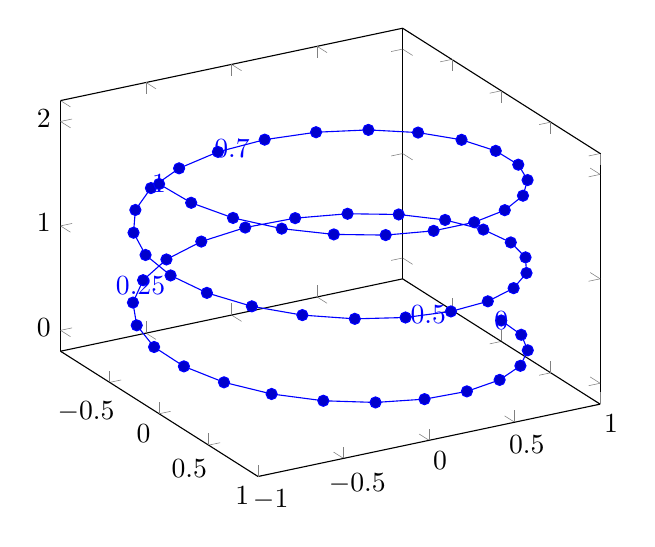
\begin{tikzpicture}
\begin{axis}[view={60}{30}]
\addplot3+[domain=0:5*pi,samples=60,samples y=0]
    ({sin(deg(x))},
     {cos(deg(x))},
     {2*x/(5*pi)})
	node[pos=0] {0} node[pos=0.25] {0.25} node[pos=0.5] {0.5} node[pos=0.7] {0.7} node[pos=1] {1};
\end{axis}
\end{tikzpicture}


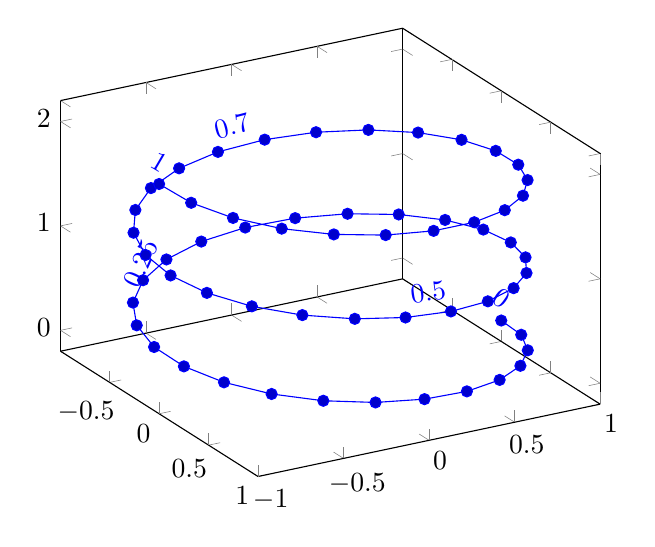
\begin{tikzpicture}
%\tracingcommands=2\tracingmacros=2
\begin{axis}[view={60}{30}]
\addplot3+[domain=0:5*pi,samples=60,samples y=0]
    ({sin(deg(x))},
     {cos(deg(x))},
     {2*x/(5*pi)})
	 [/tikz/sloped,yshift=8pt]
	node[pos=0] {0} node[pos=0.25] {0.25} node[pos=0.5] {0.5} node[pos=0.7] {0.7} node[pos=1] {1};
\end{axis}
\end{tikzpicture}
\end{document}

